\documentclass{beamer}

\usepackage{tikz}

\title{Quick Sort}
\subtitle{Sorting Algorithm}
\author{Charles Carter}
\institute{Auburn University}
\date{\today}

\begin{document}

\frame{\titlepage}

\begin{frame}
\frametitle{Table of Contents}
\tableofcontents
\end{frame}

\section{Introduction}
\begin{frame}
    \LARGE Introduction
\end{frame}

    \begin{frame}
        \frametitle{Why would we ever want to sort anything?}
        \LARGE Sorting: arranging objects in some sort of order
        \normalsize
        \begin{itemize}
            \item Integers: in numerical order, e.g., 1, 2, 3, 4, 5
            \item Characters: in alphabetical order, e.g. A, B, C, D, E
            \item Students: in class rank order
            \item Movies: in review order, highest to lowest
            \item Dates: ???
        \end{itemize}
    \end{frame}

    \begin{frame}
        \frametitle{A motivational example}
        \Large How do you finding a name in a large directory?
        \normalsize
        What if the names are not sorted?\\
        Do you start at the beginning and search until you find the name you are looking for?\\
        What if there are 1,000,000 names in the directory?\\
        The complexity of bisection search is $O = \log_2 n$
        \begin{itemize}
            \item 4 guesses to find an item in a list of size 10
            \item 7 guesses  in a list of size 100
            \item 10 guesses  in a list of size 1000
            \item 20 guesses  in a list of size 1000000
            \item 30 guesses  in a list of size 1000000000
            \item 40 guesses  in a list of size 1000000000000
        \end{itemize}
    \end{frame}

    \begin{frame}
        \frametitle{Conceptual View of QuickSort}
        \begin{itemize}
            \item A list of length 0 or 1 is ``sorted.'' Why?
            \item A list of length greater than 1 can be split in the ``middle'' and each ``half'' can be sorted. Why?
            \item Sorted lists can be combined (in order) to form a sorted list. Why?
        \end{itemize}
        \par \Large [ ] and [42] are both sorted lists.
        \par \Large [1, 2, 3] + [4, 6, 8] + [10, 20, 30] is a sorted list.
    \end{frame}

    \begin{frame}
        \frametitle{Brief Description of QuickSort}
        \begin{itemize}
            \item QuickSort is a recursive algorithm based on the ``divide and conquer'' technique. It works by placing the ``middle'' element in the proper place, i.e., in the ``middle'', and then doing the same thing for the left and right halves. This ``middle'' element is known as the \textbf{PIVOT}.
            \item Think of sorting a stack of books by number of pages. Pick a book at random (the pivot, or ``middle''), and place all the books with fewer pages on the left, and all the books with more pages on the right. Repeat for the left and right sides.
            \item Question: How would you do this for a deck of cards?
        \end{itemize}
    \end{frame}

    \begin{frame}
        \frametitle{Description of QuickSort}
        \begin{enumerate}
            \item Call the QuickSort() procedure, passing a perhaps unsorted list as the only parameter.
            \item Start with the list parameter. Pick one element of the list to be the pivot. (First, last, middle, random --- it doesn't matter.)
            \item Iterate through the list placing all elements less than the pivot on the left and all elements greater than the pivot on the right. (Equal elements can go either on the left, right, or --- in my demonstration --- in the middle.)
            \item Continue the same process for the left and right sides. Call the same procedure passing the left or right side as the parameter. This is the recursive step.
            \item Stop the recursion when a list has one or zero elements and return the list. This stops the recursion.
        \end{enumerate}
    \end{frame}

\section{Quick Sort Examples}
\begin{frame}
    \LARGE Quick Sort Examples
\end{frame}

    \begin{frame}
        \frametitle{Example 1}
            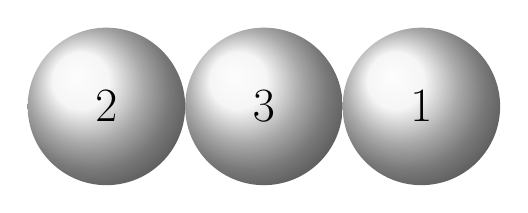
\begin{tikzpicture}
                \node[shade, shading=ball, circle, ball color=lightgray!20, minimum size=2cm] at (2,5) {\LARGE 2};
                \node[shade, shading=ball, circle, ball color=lightgray!20, minimum size=2cm] at (4,5) {\LARGE 3};
                \node[shade, shading=ball, circle, ball color=lightgray!20, minimum size=2cm] at (6,5) {\LARGE 1};
            \end{tikzpicture}
            \footnotesize Choose a pivot, use first element
            \pause
            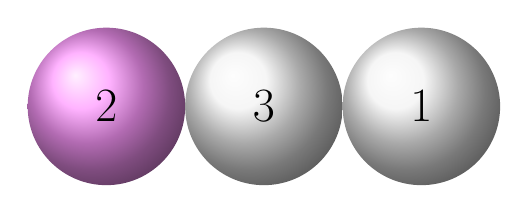
\begin{tikzpicture}
                \node[shade, shading=ball, circle, ball color=magenta!40, minimum size=2cm] at (2,3) {\LARGE 2};
                \node[shade, shading=ball, circle, ball color=lightgray!20, minimum size=2cm] at (4,3) {\LARGE 3};
                \node[shade, shading=ball, circle, ball color=lightgray!20, minimum size=2cm] at (6,3) {\LARGE 1};
            \end{tikzpicture}
            \footnotesize Sort right and left lists
            \pause
            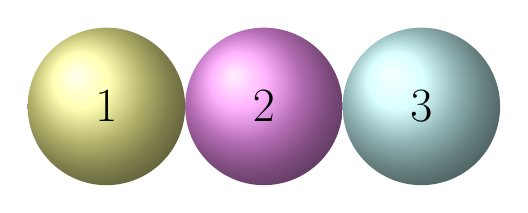
\begin{tikzpicture}
                \node[shade, shading=ball, circle, ball color=yellow!40, minimum size=2cm] at (2,3) {\LARGE 1};
                \node[shade, shading=ball, circle, ball color=magenta!40, minimum size=2cm] at (4,3) {\LARGE 2};
                \node[shade, shading=ball, circle, ball color=cyan!20, minimum size=2cm] at (6,3) {\LARGE 3};
            \end{tikzpicture}
            \footnotesize R \& L stopped, List is sorted
    \end{frame}

    \begin{frame}
        \frametitle{Example 2}
            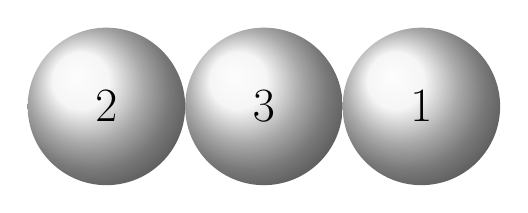
\begin{tikzpicture}
                \node[shade, shading=ball, circle, ball color=lightgray!20, minimum size=2cm] at (2,5) {\LARGE 2};
                \node[shade, shading=ball, circle, ball color=lightgray!20, minimum size=2cm] at (4,5) {\LARGE 3};
                \node[shade, shading=ball, circle, ball color=lightgray!20, minimum size=2cm] at (6,5) {\LARGE 1};
            \end{tikzpicture}
            \footnotesize Choose a pivot, use middle
            \pause
            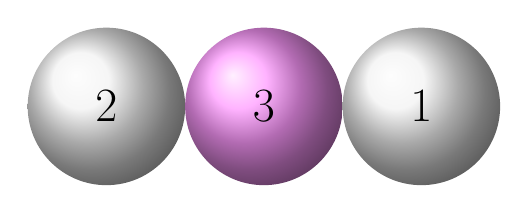
\begin{tikzpicture}
                \node[shade, shading=ball, circle, ball color=lightgray!20, minimum size=2cm] at (2,3) {\LARGE 2};
                \node[shade, shading=ball, circle, ball color=magenta!40, minimum size=2cm] at (4,3) {\LARGE 3};
                \node[shade, shading=ball, circle, ball color=lightgray!20, minimum size=2cm] at (6,3) {\LARGE 1};
            \end{tikzpicture}
            \footnotesize Sort right and left
            \pause
            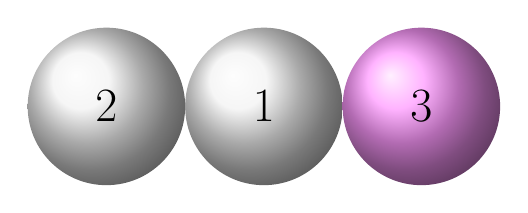
\begin{tikzpicture}
                \node[shade, shading=ball, circle, ball color=lightgray!20, minimum size=2cm] at (2,1) {\LARGE 2};
                \node[shade, shading=ball, circle, ball color=lightgray!20, minimum size=2cm] at (4,1) {\LARGE 1};
                \node[shade, shading=ball, circle, ball color=magenta!40, minimum size=2cm] at (6,1) {\LARGE 3};
            \end{tikzpicture}
            \footnotesize Sort left list
    \end{frame}

    \begin{frame}
        \frametitle{Example 2, continued}
            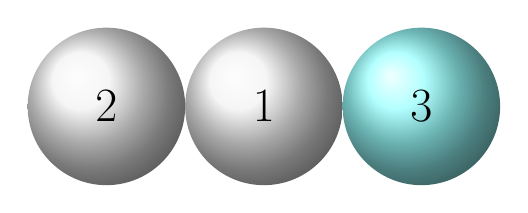
\begin{tikzpicture}
                \node[shade, shading=ball, circle, ball color=lightgray!20, minimum size=2cm] at (2,5) {\LARGE 2};
                \node[shade, shading=ball, circle, ball color=lightgray!20, minimum size=2cm] at (4,5) {\LARGE 1};
                \node[shade, shading=ball, circle, ball color=cyan!40, minimum size=2cm] at (6,5) {\LARGE 3};
            \end{tikzpicture}
            \footnotesize Choose a pivot, use middle
            \pause
            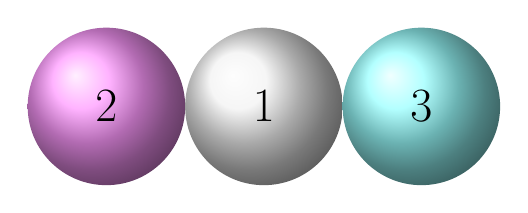
\begin{tikzpicture}
                \node[shade, shading=ball, circle, ball color=magenta!40, minimum size=2cm] at (2,3) {\LARGE 2};
                \node[shade, shading=ball, circle, ball color=lightgray!20, minimum size=2cm] at (4,3) {\LARGE 1};
                \node[shade, shading=ball, circle, ball color=cyan!40, minimum size=2cm] at (6,3) {\LARGE 3};
            \end{tikzpicture}
            \footnotesize Sort right and left
            \pause
            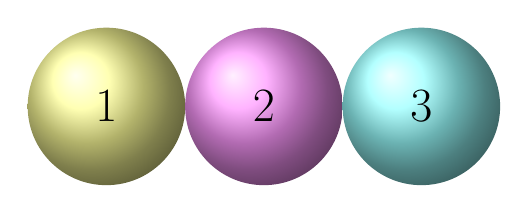
\begin{tikzpicture}
                \node[shade, shading=ball, circle, ball color=yellow!40, minimum size=2cm] at (2,-1) {\LARGE 1};
                \node[shade, shading=ball, circle, ball color=magenta!40, minimum size=2cm] at (4,-1) {\LARGE 2};
                \node[shade, shading=ball, circle, ball color=cyan!40, minimum size=2cm] at (6,-1) {\LARGE 3};
            \end{tikzpicture}
            \footnotesize List is sorted
    \end{frame}

    \begin{frame}
        \frametitle{Example 3}
            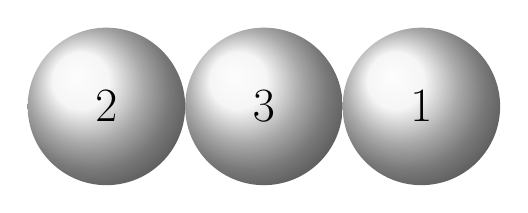
\begin{tikzpicture}
                \node[shade, shading=ball, circle, ball color=lightgray!20, minimum size=2cm] at (2,5) {\LARGE 2};
                \node[shade, shading=ball, circle, ball color=lightgray!20, minimum size=2cm] at (4,5) {\LARGE 3};
                \node[shade, shading=ball, circle, ball color=lightgray!20, minimum size=2cm] at (6,5) {\LARGE 1};
            \end{tikzpicture}
            \footnotesize Choose a pivot, use last
            \pause
            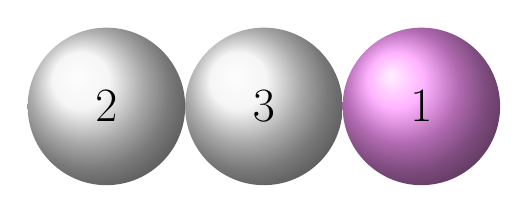
\begin{tikzpicture}
                \node[shade, shading=ball, circle, ball color=lightgray!20, minimum size=2cm] at (2,3) {\LARGE 2};
                \node[shade, shading=ball, circle, ball color=lightgray!20, minimum size=2cm] at (4,3) {\LARGE 3};
                \node[shade, shading=ball, circle, ball color=magenta!40, minimum size=2cm] at (6,3) {\LARGE 1};
            \end{tikzpicture}
            \footnotesize Sort right and left
            \pause
            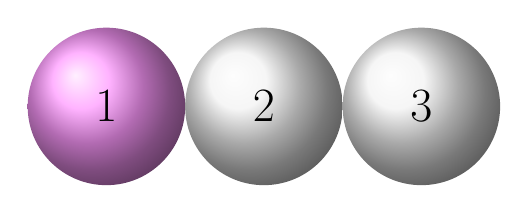
\begin{tikzpicture}
                \node[shade, shading=ball, circle, ball color=magenta!40, minimum size=2cm] at (2,3) {\LARGE 1};
                \node[shade, shading=ball, circle, ball color=lightgray!20, minimum size=2cm] at (4,3) {\LARGE 2};
                \node[shade, shading=ball, circle, ball color=lightgray!20, minimum size=2cm] at (6,3) {\LARGE 3};
            \end{tikzpicture}
            \footnotesize Sort not done, R $>$ 1
    \end{frame}

    \begin{frame}
        \frametitle{Example 3, continued}
            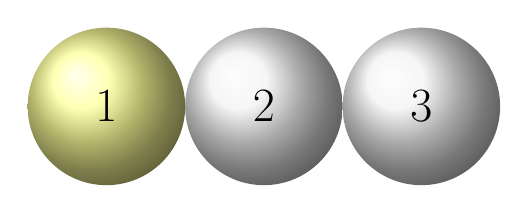
\begin{tikzpicture}
                \node[shade, shading=ball, circle, ball color=yellow!40, minimum size=2cm] at (2,3) {\LARGE 1};
                \node[shade, shading=ball, circle, ball color=lightgray!20, minimum size=2cm] at (4,3) {\LARGE 2};
                \node[shade, shading=ball, circle, ball color=lightgray!20, minimum size=2cm] at (6,3) {\LARGE 3};
            \end{tikzpicture}
            \footnotesize Choose a pivot, use last
            \pause
            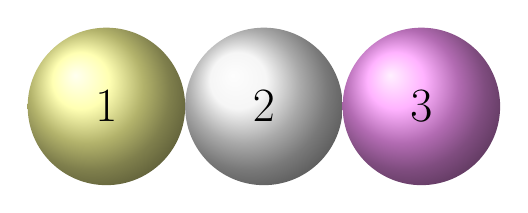
\begin{tikzpicture}
                \node[shade, shading=ball, circle, ball color=yellow!40, minimum size=2cm] at (2,3) {\LARGE 1};
                \node[shade, shading=ball, circle, ball color=lightgray!20, minimum size=2cm] at (4,3) {\LARGE 2};
                \node[shade, shading=ball, circle, ball color=magenta!40, minimum size=2cm] at (6,3) {\LARGE 3};
            \end{tikzpicture}
            \footnotesize Sorted, R == 1, L == 0
            \pause
            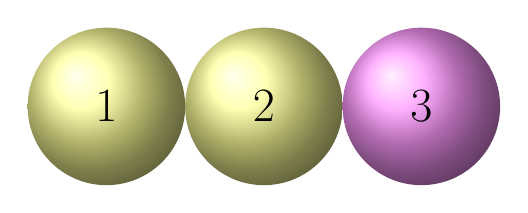
\begin{tikzpicture}
                \node[shade, shading=ball, circle, ball color=yellow!40, minimum size=2cm] at (2,3) {\LARGE 1};
                \node[shade, shading=ball, circle, ball color=yellow!40, minimum size=2cm] at (4,3) {\LARGE 2};
                \node[shade, shading=ball, circle, ball color=magenta!40, minimum size=2cm] at (6,3) {\LARGE 3};
            \end{tikzpicture}
            \footnotesize List is sorted
    \end{frame}

    \begin{frame}
        \frametitle{Extended example}
            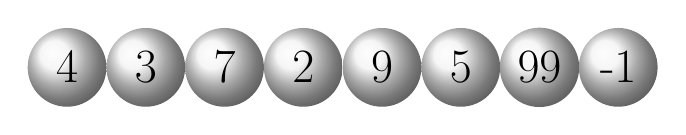
\begin{tikzpicture}
                \node[shade, shading=ball, circle, ball color=lightgray!20, minimum size=1cm] at (1,3) {\LARGE 4};
                \node[shade, shading=ball, circle, ball color=lightgray!20, minimum size=1cm] at (2,3) {\LARGE 3};
                \node[shade, shading=ball, circle, ball color=lightgray!20, minimum size=1cm] at (3,3) {\LARGE 7};
                \node[shade, shading=ball, circle, ball color=lightgray!20, minimum size=1cm] at (4,3) {\LARGE 2};
                \node[shade, shading=ball, circle, ball color=lightgray!20, minimum size=1cm] at (5,3) {\LARGE 9};
                \node[shade, shading=ball, circle, ball color=lightgray!20, minimum size=1cm] at (6,3) {\LARGE 5};
                \node[shade, shading=ball, circle, ball color=lightgray!20, minimum size=1cm] at (7,3) {\LARGE 99};
                \node[shade, shading=ball, circle, ball color=lightgray!20, minimum size=1cm] at (8,3) {\LARGE -1};
            \end{tikzpicture}
            \par Choose pivot, use middle
            \pause
            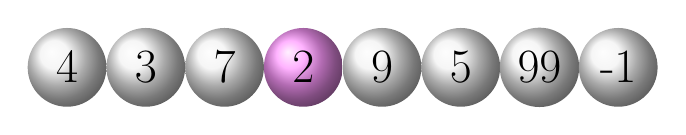
\begin{tikzpicture}
                \node[shade, shading=ball, circle, ball color=lightgray!20, minimum size=1cm] at (1,3) {\LARGE 4};
                \node[shade, shading=ball, circle, ball color=lightgray!20, minimum size=1cm] at (2,3) {\LARGE 3};
                \node[shade, shading=ball, circle, ball color=lightgray!20, minimum size=1cm] at (3,3) {\LARGE 7};
                \node[shade, shading=ball, circle, ball color=magenta!40, minimum size=1cm] at (4,3) {\LARGE 2};
                \node[shade, shading=ball, circle, ball color=lightgray!20, minimum size=1cm] at (5,3) {\LARGE 9};
                \node[shade, shading=ball, circle, ball color=lightgray!20, minimum size=1cm] at (6,3) {\LARGE 5};
                \node[shade, shading=ball, circle, ball color=lightgray!20, minimum size=1cm] at (7,3) {\LARGE 99};
                \node[shade, shading=ball, circle, ball color=lightgray!20, minimum size=1cm] at (8,3) {\LARGE -1};
            \end{tikzpicture}
            \par Place elements $<$ pivot on L, elements $>$ pivot on R
            \pause
            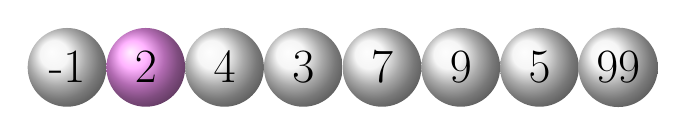
\begin{tikzpicture}
                \node[shade, shading=ball, circle, ball color=lightgray!20, minimum size=1cm] at (1,3) {\LARGE -1};
                \node[shade, shading=ball, circle, ball color=magenta!40, minimum size=1cm] at (2,3) {\LARGE 2};
                \node[shade, shading=ball, circle, ball color=lightgray!20, minimum size=1cm] at (3,3) {\LARGE 4};
                \node[shade, shading=ball, circle, ball color=lightgray!20, minimum size=1cm] at (4,3) {\LARGE 3};
                \node[shade, shading=ball, circle, ball color=lightgray!20, minimum size=1cm] at (5,3) {\LARGE 7};
                \node[shade, shading=ball, circle, ball color=lightgray!20, minimum size=1cm] at (6,3) {\LARGE 9};
                \node[shade, shading=ball, circle, ball color=lightgray!20, minimum size=1cm] at (7,3) {\LARGE 5};
                \node[shade, shading=ball, circle, ball color=lightgray!20, minimum size=1cm] at (8,3) {\LARGE 99};
            \end{tikzpicture}
            \par L is sorted, length == 1
            \pause
            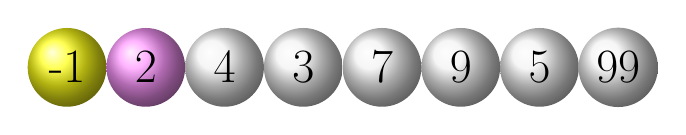
\begin{tikzpicture}
                \node[shade, shading=ball, circle, ball color=yellow!90, minimum size=1cm] at (1,3) {\LARGE -1};
                \node[shade, shading=ball, circle, ball color=magenta!40, minimum size=1cm] at (2,3) {\LARGE 2};
                \node[shade, shading=ball, circle, ball color=lightgray!20, minimum size=1cm] at (3,3) {\LARGE 4};
                \node[shade, shading=ball, circle, ball color=lightgray!20, minimum size=1cm] at (4,3) {\LARGE 3};
                \node[shade, shading=ball, circle, ball color=lightgray!20, minimum size=1cm] at (5,3) {\LARGE 7};
                \node[shade, shading=ball, circle, ball color=lightgray!20, minimum size=1cm] at (6,3) {\LARGE 9};
                \node[shade, shading=ball, circle, ball color=lightgray!20, minimum size=1cm] at (7,3) {\LARGE 5};
                \node[shade, shading=ball, circle, ball color=lightgray!20, minimum size=1cm] at (8,3) {\LARGE 99};
            \end{tikzpicture}
    \end{frame}

    \begin{frame}
        \frametitle{Extended example continued 1}
            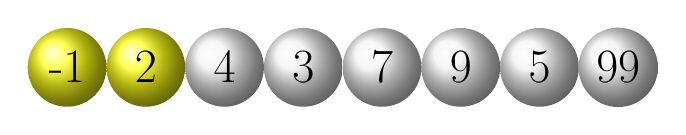
\begin{tikzpicture}
                \node[shade, shading=ball, circle, ball color=yellow!90, minimum size=1cm] at (1,3) {\LARGE -1};
                \node[shade, shading=ball, circle, ball color=yellow!90, minimum size=1cm] at (2,3) {\LARGE 2};
                \node[shade, shading=ball, circle, ball color=lightgray!20, minimum size=1cm] at (3,3) {\LARGE 4};
                \node[shade, shading=ball, circle, ball color=lightgray!20, minimum size=1cm] at (4,3) {\LARGE 3};
                \node[shade, shading=ball, circle, ball color=lightgray!20, minimum size=1cm] at (5,3) {\LARGE 7};
                \node[shade, shading=ball, circle, ball color=lightgray!20, minimum size=1cm] at (6,3) {\LARGE 9};
                \node[shade, shading=ball, circle, ball color=lightgray!20, minimum size=1cm] at (7,3) {\LARGE 5};
                \node[shade, shading=ball, circle, ball color=lightgray!20, minimum size=1cm] at (8,3) {\LARGE 99};
            \end{tikzpicture}
            \par Choose pivot, use middle
            \pause
            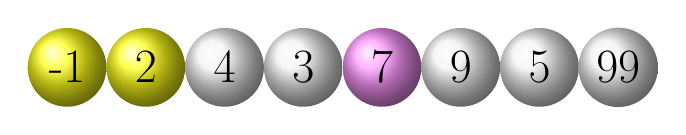
\begin{tikzpicture}
                \node[shade, shading=ball, circle, ball color=yellow!90, minimum size=1cm] at (1,3) {\LARGE -1};
                \node[shade, shading=ball, circle, ball color=yellow!90, minimum size=1cm] at (2,3) {\LARGE 2};
                \node[shade, shading=ball, circle, ball color=lightgray!20, minimum size=1cm] at (3,3) {\LARGE 4};
                \node[shade, shading=ball, circle, ball color=lightgray!20, minimum size=1cm] at (4,3) {\LARGE 3};
                \node[shade, shading=ball, circle, ball color=magenta!40, minimum size=1cm] at (5,3) {\LARGE 7};
                \node[shade, shading=ball, circle, ball color=lightgray!20, minimum size=1cm] at (6,3) {\LARGE 9};
                \node[shade, shading=ball, circle, ball color=lightgray!20, minimum size=1cm] at (7,3) {\LARGE 5};
                \node[shade, shading=ball, circle, ball color=lightgray!20, minimum size=1cm] at (8,3) {\LARGE 99};
            \end{tikzpicture}
            \par Place elements $<$ pivot on L, elements $>$ pivot on R
            \pause
            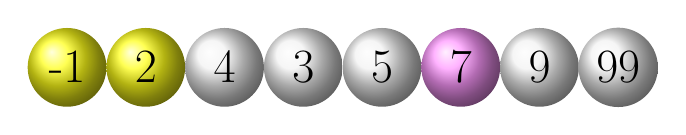
\begin{tikzpicture}
                \node[shade, shading=ball, circle, ball color=yellow!90, minimum size=1cm] at (1,3) {\LARGE -1};
                \node[shade, shading=ball, circle, ball color=yellow!90, minimum size=1cm] at (2,3) {\LARGE 2};
                \node[shade, shading=ball, circle, ball color=lightgray!20, minimum size=1cm] at (3,3) {\LARGE 4};
                \node[shade, shading=ball, circle, ball color=lightgray!20, minimum size=1cm] at (4,3) {\LARGE 3};
                \node[shade, shading=ball, circle, ball color=lightgray!20, minimum size=1cm] at (5,3) {\LARGE 5};
                \node[shade, shading=ball, circle, ball color=magenta!40, minimum size=1cm] at (6,3) {\LARGE 7};
                \node[shade, shading=ball, circle, ball color=lightgray!20, minimum size=1cm] at (7,3) {\LARGE 9};
                \node[shade, shading=ball, circle, ball color=lightgray!20, minimum size=1cm] at (8,3) {\LARGE 99};
            \end{tikzpicture}
            \par Pivot is in correct place (color is RED)
            \pause
            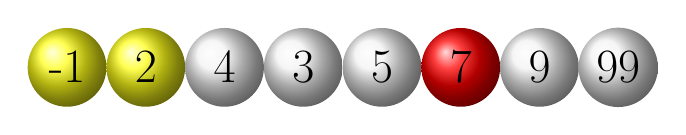
\begin{tikzpicture}
                \node[shade, shading=ball, circle, ball color=yellow!90, minimum size=1cm] at (1,3) {\LARGE -1};
                \node[shade, shading=ball, circle, ball color=yellow!90, minimum size=1cm] at (2,3) {\LARGE 2};
                \node[shade, shading=ball, circle, ball color=lightgray!20, minimum size=1cm] at (3,3) {\LARGE 4};
                \node[shade, shading=ball, circle, ball color=lightgray!20, minimum size=1cm] at (4,3) {\LARGE 3};
                \node[shade, shading=ball, circle, ball color=lightgray!20, minimum size=1cm] at (5,3) {\LARGE 5};
                \node[shade, shading=ball, circle, ball color=red, minimum size=1cm] at (6,3) {\LARGE 7};
                \node[shade, shading=ball, circle, ball color=lightgray!20, minimum size=1cm] at (7,3) {\LARGE 9};
                \node[shade, shading=ball, circle, ball color=lightgray!20, minimum size=1cm] at (8,3) {\LARGE 99};
            \end{tikzpicture}
    \end{frame}

    \begin{frame}
        \frametitle{Extended example continued 2}
            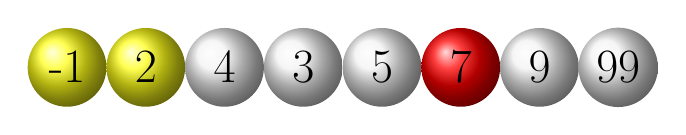
\begin{tikzpicture}
                \node[shade, shading=ball, circle, ball color=yellow!90, minimum size=1cm] at (1,3) {\LARGE -1};
                \node[shade, shading=ball, circle, ball color=yellow!90, minimum size=1cm] at (2,3) {\LARGE 2};
                \node[shade, shading=ball, circle, ball color=lightgray!20, minimum size=1cm] at (3,3) {\LARGE 4};
                \node[shade, shading=ball, circle, ball color=lightgray!20, minimum size=1cm] at (4,3) {\LARGE 3};
                \node[shade, shading=ball, circle, ball color=lightgray!20, minimum size=1cm] at (5,3) {\LARGE 5};
                \node[shade, shading=ball, circle, ball color=red, minimum size=1cm] at (6,3) {\LARGE 7};
                \node[shade, shading=ball, circle, ball color=lightgray!20, minimum size=1cm] at (7,3) {\LARGE 9};
                \node[shade, shading=ball, circle, ball color=lightgray!20, minimum size=1cm] at (8,3) {\LARGE 99};
            \end{tikzpicture}
            \par Sorting L, Choose pivot, use middle
            \pause
            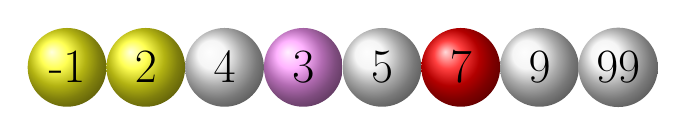
\begin{tikzpicture}
                \node[shade, shading=ball, circle, ball color=yellow!90, minimum size=1cm] at (1,3) {\LARGE -1};
                \node[shade, shading=ball, circle, ball color=yellow!90, minimum size=1cm] at (2,3) {\LARGE 2};
                \node[shade, shading=ball, circle, ball color=lightgray!20, minimum size=1cm] at (3,3) {\LARGE 4};
                \node[shade, shading=ball, circle, ball color=magenta!40, minimum size=1cm] at (4,3) {\LARGE 3};
                \node[shade, shading=ball, circle, ball color=lightgray!20, minimum size=1cm] at (5,3) {\LARGE 5};
                \node[shade, shading=ball, circle, ball color=red, minimum size=1cm] at (6,3) {\LARGE 7};
                \node[shade, shading=ball, circle, ball color=lightgray!20, minimum size=1cm] at (7,3) {\LARGE 9};
                \node[shade, shading=ball, circle, ball color=lightgray!20, minimum size=1cm] at (8,3) {\LARGE 99};
            \end{tikzpicture}
            \par Place elements $<$ pivot on L, elements $>$ pivot on R
            \pause
            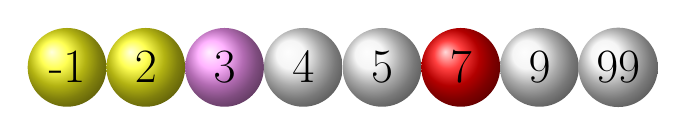
\begin{tikzpicture}
                \node[shade, shading=ball, circle, ball color=yellow!90, minimum size=1cm] at (1,3) {\LARGE -1};
                \node[shade, shading=ball, circle, ball color=yellow!90, minimum size=1cm] at (2,3) {\LARGE 2};
                \node[shade, shading=ball, circle, ball color=magenta!40, minimum size=1cm] at (3,3) {\LARGE 3};
                \node[shade, shading=ball, circle, ball color=lightgray!20, minimum size=1cm] at (4,3) {\LARGE 4};
                \node[shade, shading=ball, circle, ball color=lightgray!20, minimum size=1cm] at (5,3) {\LARGE 5};
                \node[shade, shading=ball, circle, ball color=red, minimum size=1cm] at (6,3) {\LARGE 7};
                \node[shade, shading=ball, circle, ball color=lightgray!20, minimum size=1cm] at (7,3) {\LARGE 9};
                \node[shade, shading=ball, circle, ball color=lightgray!20, minimum size=1cm] at (8,3) {\LARGE 99};
            \end{tikzpicture}
            \par L is sorted, length == 0, sort R
            \pause
            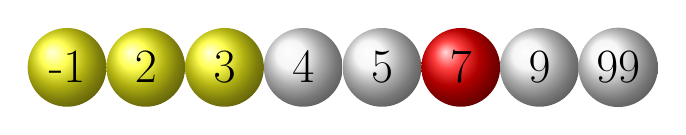
\begin{tikzpicture}
                \node[shade, shading=ball, circle, ball color=yellow!90, minimum size=1cm] at (1,3) {\LARGE -1};
                \node[shade, shading=ball, circle, ball color=yellow!90, minimum size=1cm] at (2,3) {\LARGE 2};
                \node[shade, shading=ball, circle, ball color=yellow!90, minimum size=1cm] at (3,3) {\LARGE 3};
                \node[shade, shading=ball, circle, ball color=lightgray!20, minimum size=1cm] at (4,3) {\LARGE 4};
                \node[shade, shading=ball, circle, ball color=lightgray!20, minimum size=1cm] at (5,3) {\LARGE 5};
                \node[shade, shading=ball, circle, ball color=red, minimum size=1cm] at (6,3) {\LARGE 7};
                \node[shade, shading=ball, circle, ball color=lightgray!20, minimum size=1cm] at (7,3) {\LARGE 9};
                \node[shade, shading=ball, circle, ball color=lightgray!20, minimum size=1cm] at (8,3) {\LARGE 99};
            \end{tikzpicture}
    \end{frame}

    \begin{frame}
        \frametitle{Extended example continued 3}
            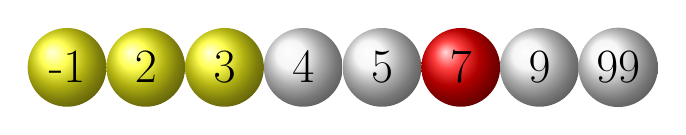
\begin{tikzpicture}
                \node[shade, shading=ball, circle, ball color=yellow!90, minimum size=1cm] at (1,3) {\LARGE -1};
                \node[shade, shading=ball, circle, ball color=yellow!90, minimum size=1cm] at (2,3) {\LARGE 2};
                \node[shade, shading=ball, circle, ball color=yellow!90, minimum size=1cm] at (3,3) {\LARGE 3};
                \node[shade, shading=ball, circle, ball color=lightgray!20, minimum size=1cm] at (4,3) {\LARGE 4};
                \node[shade, shading=ball, circle, ball color=lightgray!20, minimum size=1cm] at (5,3) {\LARGE 5};
                \node[shade, shading=ball, circle, ball color=red, minimum size=1cm] at (6,3) {\LARGE 7};
                \node[shade, shading=ball, circle, ball color=lightgray!20, minimum size=1cm] at (7,3) {\LARGE 9};
                \node[shade, shading=ball, circle, ball color=lightgray!20, minimum size=1cm] at (8,3) {\LARGE 99};
            \end{tikzpicture}
            \par Choose pivot, use middle
            \pause
            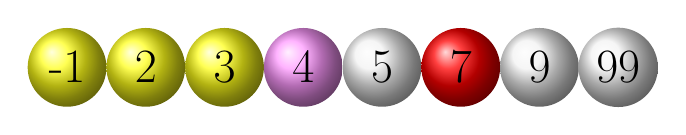
\begin{tikzpicture}
                \node[shade, shading=ball, circle, ball color=yellow!90, minimum size=1cm] at (1,3) {\LARGE -1};
                \node[shade, shading=ball, circle, ball color=yellow!90, minimum size=1cm] at (2,3) {\LARGE 2};
                \node[shade, shading=ball, circle, ball color=yellow!90, minimum size=1cm] at (3,3) {\LARGE 3};
                \node[shade, shading=ball, circle, ball color=magenta!40, minimum size=1cm] at (4,3) {\LARGE 4};
                \node[shade, shading=ball, circle, ball color=lightgray!20, minimum size=1cm] at (5,3) {\LARGE 5};
                \node[shade, shading=ball, circle, ball color=red, minimum size=1cm] at (6,3) {\LARGE 7};
                \node[shade, shading=ball, circle, ball color=lightgray!20, minimum size=1cm] at (7,3) {\LARGE 9};
                \node[shade, shading=ball, circle, ball color=lightgray!20, minimum size=1cm] at (8,3) {\LARGE 99};
            \end{tikzpicture}
            \par L is sorted, length == 0
            \pause
            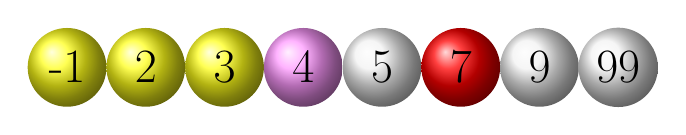
\begin{tikzpicture}
                \node[shade, shading=ball, circle, ball color=yellow!90, minimum size=1cm] at (1,3) {\LARGE -1};
                \node[shade, shading=ball, circle, ball color=yellow!90, minimum size=1cm] at (2,3) {\LARGE 2};
                \node[shade, shading=ball, circle, ball color=yellow!90, minimum size=1cm] at (3,3) {\LARGE 3};
                \node[shade, shading=ball, circle, ball color=magenta!40, minimum size=1cm] at (4,3) {\LARGE 4};
                \node[shade, shading=ball, circle, ball color=lightgray!20, minimum size=1cm] at (5,3) {\LARGE 5};
                \node[shade, shading=ball, circle, ball color=red, minimum size=1cm] at (6,3) {\LARGE 7};
                \node[shade, shading=ball, circle, ball color=lightgray!20, minimum size=1cm] at (7,3) {\LARGE 9};
                \node[shade, shading=ball, circle, ball color=lightgray!20, minimum size=1cm] at (8,3) {\LARGE 99};
            \end{tikzpicture}
            \par R is sorted, length == 1
            \pause
            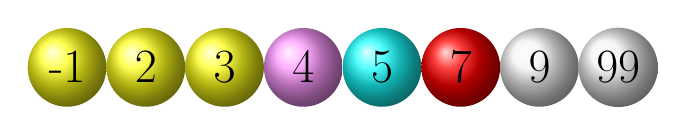
\begin{tikzpicture}
                \node[shade, shading=ball, circle, ball color=yellow!90, minimum size=1cm] at (1,3) {\LARGE -1};
                \node[shade, shading=ball, circle, ball color=yellow!90, minimum size=1cm] at (2,3) {\LARGE 2};
                \node[shade, shading=ball, circle, ball color=yellow!90, minimum size=1cm] at (3,3) {\LARGE 3};
                \node[shade, shading=ball, circle, ball color=magenta!40, minimum size=1cm] at (4,3) {\LARGE 4};
                \node[shade, shading=ball, circle, ball color=cyan!90, minimum size=1cm] at (5,3) {\LARGE 5};
                \node[shade, shading=ball, circle, ball color=red, minimum size=1cm] at (6,3) {\LARGE 7};
                \node[shade, shading=ball, circle, ball color=lightgray!20, minimum size=1cm] at (7,3) {\LARGE 9};
                \node[shade, shading=ball, circle, ball color=lightgray!20, minimum size=1cm] at (8,3) {\LARGE 99};
            \end{tikzpicture}
    \end{frame}

    \begin{frame}
        \frametitle{Extended example continued 4}
            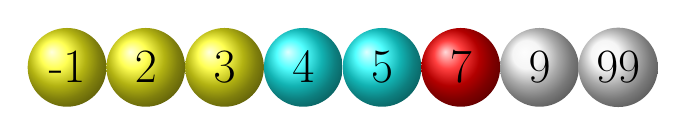
\begin{tikzpicture}
                \node[shade, shading=ball, circle, ball color=yellow!90, minimum size=1cm] at (1,3) {\LARGE -1};
                \node[shade, shading=ball, circle, ball color=yellow!90, minimum size=1cm] at (2,3) {\LARGE 2};
                \node[shade, shading=ball, circle, ball color=yellow!90, minimum size=1cm] at (3,3) {\LARGE 3};
                \node[shade, shading=ball, circle, ball color=cyan!90, minimum size=1cm] at (4,3) {\LARGE 4};
                \node[shade, shading=ball, circle, ball color=cyan!90, minimum size=1cm] at (5,3) {\LARGE 5};
                \node[shade, shading=ball, circle, ball color=red, minimum size=1cm] at (6,3) {\LARGE 7};
                \node[shade, shading=ball, circle, ball color=lightgray!20, minimum size=1cm] at (7,3) {\LARGE 9};
                \node[shade, shading=ball, circle, ball color=lightgray!20, minimum size=1cm] at (8,3) {\LARGE 99};
            \end{tikzpicture}
            \par Choose pivot, use middle
            \pause
            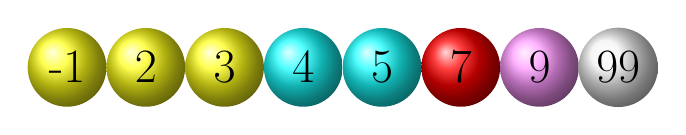
\begin{tikzpicture}
                \node[shade, shading=ball, circle, ball color=yellow!90, minimum size=1cm] at (1,3) {\LARGE -1};
                \node[shade, shading=ball, circle, ball color=yellow!90, minimum size=1cm] at (2,3) {\LARGE 2};
                \node[shade, shading=ball, circle, ball color=yellow!90, minimum size=1cm] at (3,3) {\LARGE 3};
                \node[shade, shading=ball, circle, ball color=cyan!90, minimum size=1cm] at (4,3) {\LARGE 4};
                \node[shade, shading=ball, circle, ball color=cyan!90, minimum size=1cm] at (5,3) {\LARGE 5};
                \node[shade, shading=ball, circle, ball color=red, minimum size=1cm] at (6,3) {\LARGE 7};
                \node[shade, shading=ball, circle, ball color=magenta!40, minimum size=1cm] at (7,3) {\LARGE 9};
                \node[shade, shading=ball, circle, ball color=lightgray!20, minimum size=1cm] at (8,3) {\LARGE 99};
            \end{tikzpicture}
            \par L is sorted, length == 0
            \pause
            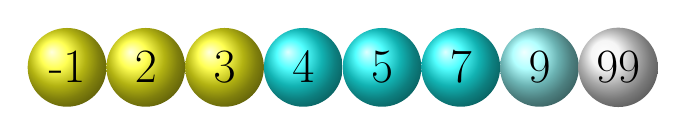
\begin{tikzpicture}
                \node[shade, shading=ball, circle, ball color=yellow!90, minimum size=1cm] at (1,3) {\LARGE -1};
                \node[shade, shading=ball, circle, ball color=yellow!90, minimum size=1cm] at (2,3) {\LARGE 2};
                \node[shade, shading=ball, circle, ball color=yellow!90, minimum size=1cm] at (3,3) {\LARGE 3};
                \node[shade, shading=ball, circle, ball color=cyan!90, minimum size=1cm] at (4,3) {\LARGE 4};
                \node[shade, shading=ball, circle, ball color=cyan!90, minimum size=1cm] at (5,3) {\LARGE 5};
                \node[shade, shading=ball, circle, ball color=cyan!90, minimum size=1cm] at (6,3) {\LARGE 7};
                \node[shade, shading=ball, circle, ball color=cyan!40, minimum size=1cm] at (7,3) {\LARGE 9};
                \node[shade, shading=ball, circle, ball color=lightgray!20, minimum size=1cm] at (8,3) {\LARGE 99};
            \end{tikzpicture}
            \par R is sorted, length == 1
            \pause
            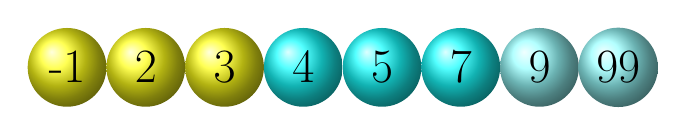
\begin{tikzpicture}
                \node[shade, shading=ball, circle, ball color=yellow!90, minimum size=1cm] at (1,3) {\LARGE -1};
                \node[shade, shading=ball, circle, ball color=yellow!90, minimum size=1cm] at (2,3) {\LARGE 2};
                \node[shade, shading=ball, circle, ball color=yellow!90, minimum size=1cm] at (3,3) {\LARGE 3};
                \node[shade, shading=ball, circle, ball color=cyan!90, minimum size=1cm] at (4,3) {\LARGE 4};
                \node[shade, shading=ball, circle, ball color=cyan!90, minimum size=1cm] at (5,3) {\LARGE 5};
                \node[shade, shading=ball, circle, ball color=cyan!90, minimum size=1cm] at (6,3) {\LARGE 7};
                \node[shade, shading=ball, circle, ball color=cyan!40, minimum size=1cm] at (7,3) {\LARGE 9};
                \node[shade, shading=ball, circle, ball color=cyan!40, minimum size=1cm] at (8,3) {\LARGE 99};
            \end{tikzpicture}
    \end{frame}

\section{Demonstration}
\begin{frame}
    \LARGE Demonstration
\end{frame}

    \begin{frame}[fragile]
        \frametitle{Python code}
        \footnotesize
        \begin{verbatim}
def quick_sort(arr):
    less = []
    equal = []
    more = []
    if len(arr) <= 1:
        return arr
    else:
        pivot = arr[(len(arr)-1) // 2]
        for i in arr:
            if i < pivot:           
                less.append(i)
            elif i > pivot:
                more.append(i)
            else:
                equal.append(i)
        less = quick_sort(less)
        more = quick_sort(more)
        return less + equal + more
        \end{verbatim}
    \end{frame}

    \begin{frame}[fragile]
        \frametitle{Python code comments, declare variables}
        \begin{verbatim}
def quick_sort(arr):
    less = []
    equal = []
    more = []
        \end{verbatim}
        \par Declare a function named \textit{quick\_sort} that takes one parameter, a list, which presumably is unsorted.
        \par Declare a \textit{less} list to hold the lesser-than items, a \textit{more} list to hold the greater-than items, and an \textit{equal} lost to hold the equal-to items.
    \end{frame}

    \begin{frame}[fragile]
        \frametitle{Python code}
        \footnotesize
        \begin{verbatim}
    if len(arr) <= 1:
        return arr
    else:
        \end{verbatim}
        \par If the length of the parameter list is 1 or 0, you are done. Stop the recursion.
        \par Else, continue the recursion.
    \end{frame}

    \begin{frame}[fragile]
        \frametitle{Python code}
        \footnotesize
        \begin{verbatim}
        pivot = arr[(len(arr)-1) // 2] #select the middle element
        for i in arr:
            if i < pivot:           
                less.append(i)
            elif i > pivot:
                more.append(i)
            else:
                equal.append(i)
        \end{verbatim}
        \par Select a pivot. It could be the first element (\textit{arr[0]}), the last element (\textit{arr[-1]}), the middle element (\textit{arr[len(arr)-1 // 2]}), or a random element.
        \par Iterate through the parameter list, placing all lesser-than elements on the left, and all greater than elements on the right.
    \end{frame}

    \begin{frame}[fragile]
        \frametitle{Python code}
        \footnotesize
        \begin{verbatim}
        #recursive calls for the right and left lists
        less = quick_sort(less)
        more = quick_sort(more)

        #return the left, middle, and right lists glued together
        return less + equal + more
        \end{verbatim}
        \par Call the function recursively on the left and right sides, passing each as a parameter. Return the three lists glued together.
    \end{frame}

    \begin{frame}[fragile]
        \frametitle{QuickSort output 1}
        \scriptsize
        \begin{verbatim}
initial list is [4, 3, 7, 2, 9, 5, 99, -1]
calling quick_sort([4, 3, 7, 2, 9, 5, 99, -1])
    else branch, list is [4, 3, 7, 2, 9, 5, 99, -1]
       for: i = 4 and pivot = 2, i > pivot, more = [4]
       for: i = 3 and pivot = 2, i > pivot, more = [4, 3]
       for: i = 7 and pivot = 2, i > pivot, more = [4, 3, 7]
       for: i = 2 and pivot = 2, i == pivot, equal = [2]
       for: i = 9 and pivot = 2, i > pivot, more = [4, 3, 7, 9]
       for: i = 5 and pivot = 2, i > pivot, more = [4, 3, 7, 9, 5]
       for: i = 99 and pivot = 2, i > pivot, more = [4, 3, 7, 9, 5, 99]
       for: i = -1 and pivot = 2, i < pivot, less = [-1]
        \end{verbatim}
    \end{frame}

    \begin{frame}[fragile]
        \frametitle{QuickSort output 1}
        \scriptsize
        \begin{verbatim}
calling quick_sort([-1])
    DONE if list length <= 1, returning [-1]
calling quick_sort([4, 3, 7, 9, 5, 99])
    else branch, list is [4, 3, 7, 9, 5, 99]
       for: i = 4 and pivot = 7, i < pivot, less = [4]
       for: i = 3 and pivot = 7, i < pivot, less = [4, 3]
       for: i = 7 and pivot = 7, i == pivot, equal = [7]
       for: i = 9 and pivot = 7, i > pivot, more = [9]
       for: i = 5 and pivot = 7, i < pivot, less = [4, 3, 5]
       for: i = 99 and pivot = 7, i > pivot, more = [9, 99]
        \end{verbatim}
    \end{frame}

    \begin{frame}[fragile]
        \frametitle{QuickSort output 1}
        \scriptsize
        \begin{verbatim}
calling quick_sort([4, 3, 5])
    else branch, list is [4, 3, 5]
       for: i = 4 and pivot = 3, i > pivot, more = [4]
       for: i = 3 and pivot = 3, i == pivot, equal = [3]
       for: i = 5 and pivot = 3, i > pivot, more = [4, 5]
calling quick_sort([])
    DONE if list length <= 1, returning []
calling quick_sort([4, 5])
    else branch, list is [4, 5]
       for: i = 4 and pivot = 4, i == pivot, equal = [4]
       for: i = 5 and pivot = 4, i > pivot, more = [5]
calling quick_sort([])
    DONE if list length <= 1, returning []
        \end{verbatim}
    \end{frame}

    \begin{frame}[fragile]
        \frametitle{QuickSort output 1}
        \scriptsize
        \begin{verbatim}
calling quick_sort([5])
    DONE if list length <= 1, returning [5]
<<<returning [] + [4] + [5]
<<<returning [] + [3] + [4, 5]
calling quick_sort([9, 99])
    else branch, list is [9, 99]
       for: i = 9 and pivot = 9, i == pivot, equal = [9]
       for: i = 99 and pivot = 9, i > pivot, more = [99]
calling quick_sort([])
    DONE if list length <= 1, returning []
calling quick_sort([99])
    DONE if list length <= 1, returning [99]
<<<returning [] + [9] + [99]
<<<returning [3, 4, 5] + [7] + [9, 99]
<<<returning [-1] + [2] + [3, 4, 5, 7, 9, 99]
end list is [-1, 2, 3, 4, 5, 7, 9, 99]
        \end{verbatim}
    \end{frame}

\section{Conclusion Questions}
\begin{frame}
    \LARGE Conclusion and Questions
\end{frame}

    \begin{frame}
        \frametitle{Time complexity of QuickSort}
        \par Best case
        \begin{equation}
            O = n \log_2 n
        \end{equation}
        \par Worst case
        \begin{equation}
            O = n^2
        \end{equation}

    \end{frame}

%    \begin{frame}
%        \frametitle{History of QuickSort}
%
%    \end{frame}
%
%    \begin{frame}
%        \frametitle{Alternatives to QuickSort}
%
%    \end{frame}

    \begin{frame}
        \frametitle{Questions}

    \end{frame}


\end{document}
